\documentclass{article}
\usepackage[utf8]{inputenc}
\usepackage[a4paper, margin=0.9in, 10pt]{geometry}
\usepackage{amsmath, amssymb}
\usepackage{algorithm, algorithmic}
\usepackage{graphicx}
\usepackage{hyperref}
\usepackage{xcolor}
\usepackage{float}

\title{CSC373 A1}
\author{Isaac Ng, Nathan Chao, Jean Li}
\date{October 13, 2020}

\newcommand{\bigO}{\mathcal{O}}

\begin{document}

\maketitle
\begin{enumerate}
    \item % ====== QUESTION 1 =======
%     \begin{enumerate}
%         \item We need two arrays to store information from subproblems, $p$ and $OPT$. Our set of gardens is sorted by easiness (non-decreasing order) before we calculate $p$. Let $p[j] =$ the largest index $i<j$ such that garden $j$ is a smarter choice than garden $i$ (i.e., $e_j > e_i \wedge q_j > q_i$). Let $OPT[j] =$ the maximum total weight of any chain of gardens chosen from gardens $\{1, ..., j\}$. 
        
%         For our final answer, we want to find $OPT[n]$.
%         \item \textbf{Bellman equation.}
%         \[
%             OPT[j]=
%             \begin{cases}
%                0 & \text{if $j=0$}\\
%                max\{OPT[j-1], w_j + OPT[p[j]]\} & \text{if $j>0$}
%             \end{cases}
%         \]
%         \textbf{Justification.} Consider an optimal solution (chain of maximum weight). If garden $j$ is not in that optimal chain, then $OPT[j]=OPT[j-1]$. If garden $j$ is in that optimal chain, then we should add $w_j$ to the maximum weight chain which consists of gardens from $\{1, ..., p[j]\}$. Note that $j$ is a smarter choice than these gardens (by the definition of $p$), so the sequence created by appending garden $j$ still meets Bobby's definition of a chain.
%         \item \textbf{Bottom-up implementation.}
%         \begin{enumerate}
%             \item Sort the $n$ given gardens by their easiness in non-decreasing order. Let the gardens be labelled $\{1, ..., n\}$ in this order. 
%             \item Initiate an array $p$. For each garden $j$ from 1 to $n$, calculate $p[j]$ (according to the definition given in part (a)) using binary search.
%             \item Initiate an array $OPT$. For each garden $j$ from $1$ to $n$, calculate $OPT[j]$ according to the Bellman equation in part (b).
%             \item Initiate an array $optchain$. If $OPT[n]=0$, return $optchain$ (empty array), since there are no chains in the garden (gardens have non-negative weights).
            
%             Otherwise, $OPT[n] > 0$, so the chain has at least one garden. In order to determine which gardens are in the optimal chain, check each garden again from $1$ to $n$. If $OPT[j-1] > w_j + OPT[p[j]]$, then garden $j$ is not in the chain. Otherwise, if $w_j + OPT[p[j]] \geq OPT[j-1]$, garden $j$ is in the chain, so append $j$ to $optchain$.
%             \item Finally, once we have considered all $n$ gardens, return $optchain$.
%         \end{enumerate}
%         \item \textbf{Running time.} Step i of the algorithm takes $\bigO(n \log n)$ time. Step ii takes $\bigO(n \log n)$ time, since $n$ binary searches are performed. Steps iii takes $\bigO(n)$ time, since $OPT[j]$ needs to be computed no more than one time for each of $j \in \{1, ..., n\}$, and each computation takes constant time. Step v takes constant time. Therefore, the total running time of the algorithm is $\bigO(n \log n)$.
        
%         \textbf{Space complexity.} Arrays $p$ and $OPT$ each have one entry for every garden. Thus, the space complexity of the algorithm is $\bigO(n)$.
%     \end{enumerate}
    
%     \newpage
%    Isaac attempt at question 1\\
    \begin{enumerate}
        \item We need two arrays to store information from sub-problems, $p$ and $OPT$. Our set of gardens is first sorted by easiness (non-decreasing order). For list $p$, let $p[j]$ be the set of end points of an increasing run in terms of quantities of gardens in the sorted list between $\{ 1, ..., j-1\}$. Note that a run does not necessarily contain only consecutive gardens (ex. $\{1, 2, 3\}$ is a run in $\{1, 7, 2, 3\}$). Before we explain the end points, remember that this is sorted by easiness already so, by definition, if we choose any garden before garden $j$, one of the two conditions for it to be smarter is already fulfilled.
        
        In order to explain the set of end points of an increasing run in terms of quantity, let's isolate a set of quantities of fruits from each garden, say $q=\{1, 9, 11, 3, 4, 2, 6, 10\}$. Let us look at the last index, $j=8$, which has the fruit quantity value $q_8=10$. The end points with increasing runs would be the indices for fruit quantities $\{11, 6\}$, which are at indices $\{3, 7\}$. These are the values where, between indices $\{1, ..., j-1\}$, there are no larger indices with larger fruit quantity values. We then make sure there are no ends of runs which are larger than $q_j$ in a separate for loop.
        
        Pseudo-code to find array $p$ with $g$ representing gardens:\\
        for $i$ in 1 to $n$
        \begin{itemize}
            \item if $i$ == 1
            \begin{itemize}
                \item $p[i]$ = []
            \end{itemize}
            \item else
            \begin{itemize}
            							\item $p[i] = p[i-1]$
                \item from $p[i]$, remove gardens with fruit quantity smaller than $q_{i-1}$ and add garden $g_{i-1}$
            \end{itemize}
        \end{itemize}
        for $i$ in 1 to $n$
        \begin{itemize}
            \item while $max_{x\in p[i]}\{p[i]\} > q_i$
            \begin{itemize}
                \item remove $max_{x\in p[i]}\{p[i]\}$ and append $p[max_{x\in p[i]}\{p[i]\}]$
            \end{itemize}
        \end{itemize}
        
        \\
        Let $OPT[j]$ be the maximum total weight of any chain of gardens containing and ending at garden $j$. This means the chain contains gardens from the set $\{ 1, ..., j\}$. $OPT[j]$ is a bottom up algorithm which starts at the first garden 1. $p[j]$ helps identify which previously calculated chains we should look at to calculate $OPT[j]$.
        
        Pseudo-code to find array $OPT$ with g representing gardens:\\ $compute$-$opt(j)$:\\
        if $p[j] = []$
        \begin{itemize}
            \item return $w_j$
        \end{itemize}
        else
        \begin{itemize}
            \item return $max_{x \in p[j]}\{w_j + OPT[x]\}$
        \end{itemize}
        For our final answer, we want to find the maximum in the array $OPT$. Then, starting with $j$ as the index with the max value of $OPT$, use $max_{x \in p[j]} \{OPT[x]\}$ repeatedly to find the previous member in the maximum weighted chain.
        
        \newpage
        \item \textbf{Bellman equation.}
        \[
            OPT[j]=
            \begin{cases}
               0 & \text{if $j=0$}\\
               max_{x \in p[j]}\{w_j + OPT[x]\} & \text{if $j>0$} 
            \end{cases}
        \]
        \textbf{Justification.} Consider an optimal solution which contains garden $j$. We want to add garden $j$ to a chain of other gardens from $1, ... j-1$ in order to have the largest weighted chain containing $j$.\\
        We notice that we do not need to check the optimal chain of each and every garden $\{1, ..., j-1\}$ because if a garden is within a 'run', since all weights are positive, we know that we should add the gardens within each 'run' to maximize the weight of that chain. There are cases with multiple possibilities to add onto a chain. As seen with our example above, 10 can either be added onto the 'run' ending at 9 or the 'run' ending at 6. This algorithm finds the maximum between the two and adds 10 onto that chain to get $OPT[j]$.This will provide us with what Bobby is looking for from the set of gardens 1 to j when the condition that garden $j$ must be in the chain.\\
        
        \item \textbf{Bottom-up implementation}
        \begin{enumerate}
            \item Sort the $n$ given gardens by their easiness in non-decreasing order. Let the gardens be labelled $\{ 1, ..., n\}$ in this order.
            \item Initiate an array $p$. For each garden $j$ from 1 to $n$, calculate $p[j]$ according to the code given in part (a).
            \item Initiate an array $OPT$. For each garden $j$ from 1 to $n$, calculate $OPT[j]$ according to the equation in part (b).
            \item Find the max value in the array $OPT$.
            \item Starting with $j$ as the index with the max value of $OPT$, use $max_{x \in p[j]} \{OPT[x]\}$ repeatedly to find the previous member in the maximum weighted chain.
        \end{enumerate}
        
        \item \textbf{Running time.} The running time of step i is in $\mathcal{O}(n\log n)$. The running time of step ii is in $\mathcal{O}(n + n*n) = \mathcal{O}(n^2)$. Both for loops run $n$ times and the while loop in the second for loop can run at most $n$ times. For step iii, we use a bottom-up approach, and each element in $OPT$ only needs to be computed one time. Finding the maximum among constants takes constant time so, the running time for step iii is $\mathcal{O}(n)$. Step iv takes constant time since we are finding the maximum among integers. Step v is similar to step iii and takes $\mathcal{O}(n)$ time. This means the overall running time complexity is in $\mathcal{O}(n^2)$.
        
        \textbf{Space complexity.} Array $p$ has at most $i$ entries at index $i$ and array $OPT$ has one entry for each garden. Therefore, the space complexity of the algorithm is $(\sum^n_{i=1} i) + n = \frac{n(n-1)}{2} + n = \mathcal{O}(n^2)$.
     \end{enumerate}
    
    
    \newpage
    \item % ====== QUESTION 2 =======
    \begin{enumerate}
        \item 
        Note: I used a sparse table. Reference: \href{https://www.youtube.com/watch?v=c5O7E_PDO4U&ab_channel=TusharRoy-CodingMadeSimple}{\color{blue}{Click Here}}\\
        \\
        Assume that giraffes are indexed $0, 1, ..., n - 1$.\\
        \\
        The table DP that I would pre-compute would have $n$ rows and $\lfloor \log(n) \rfloor + 1$ columns.\\
        \\
        The entry in DP[i][j] would be the index of the tallest giraffe with an index in the inclusive range $[i, i + 2^j - 1]$. This is the maximum of the sub-array of $H$ with length $2^j$ that starts at index $i$. Some entries in the bottom right of the table are not possible to be computed because the sub-array that they consider is not valid.\\
        \\
        For a query for giraffes $i$ through $j$:\\ First, find the ``length" of the query. Denote the length with $l = j - i + 1$.\\ Then, calculate $k = \lfloor \log(l)\rfloor$.\\ Lookup \textit{first\_max} = DP[i][k] to find the maximum of the first $2^k$ giraffes in the query.\\ Let $remaining = l - 2^k$ be the number of giraffes at the end of the query range that we haven't checked yet (\textit{remaining} could be 0). To check the last $remaining = l - 2^k$ giraffes, lookup \textit{second\_max} = DP[i + $remaining$][$k$].\\ Then the maximum of the whole query will be the maximum of $first\_max$ and $second\_max$. \\ \\ \textbf{Runtime:} \\This query takes constant time because there's $\mathcal{O}(1)$ operations that each take $\mathcal{O}(1)$ time. \\ \textbf{Correctness:} \\ $first\_max$ is the maximum height of the first $2^k$ giraffes in the range [i, j]. \textit{second\_max} is the maximum height of giraffes in the range\begin{align*}
        [i + remaining, i + remaining + 2^k - 1] &= [i + (l - 2^k), i + (l - 2^k) + 2^k - 1] \\
        &= [i + l - 2^k, i + l - 1] \\
        &= [i + (j - i+ 1) - 2^k, i + (j - i+ 1) - 1] \\
        &= [j + 1 - 2^k, j] \\
        \end{align*} This shows that $second\_max$ is the maximum height of the last $2^k$ giraffes in the range [i, j]. This means we just need to prove that all giraffes in the interval [i, j] are either in the first $2^k$ giraffes of the interval or in the last $2^k$ giraffes in the interval because then the tallest giraffe will be $first\_max$ or $second\_max$. Assume for a contradiction that there's a giraffe $m$ that's in the interval [i, j] but not in the first $2^k$ giraffes or last $2^k$ giraffes of the interval. Then there must be more than $2(2^k)$ giraffes in the interval. Recall that $l = j - i + 1$. This means \begin{align*}
    l  &> 2(2^{k})\\
    &= 2(2^{\lfloor \log(l)\rfloor})\\ 
   \end{align*}
    But then $l > 2l$ which is a contradiction. Therefore all giraffes in the interval [i, j] are in the first or last $2^k$ giraffes of the interval and so the algorithm is correct.
    
    \newpage
    \item
    \[ DP[i][j] = \begin{cases} 
      i & j = 0 \\
       DP[i][j - 1] &j \neq 0 \text{ and } H[DP[i][j - 1]]  > H[DP[i + 2^{j-1}][j-1]]\\
       DP[i + 2^{j-1}][j-1] &j \neq 0 \text{ and } H[DP[i][j - 1]]  \leq H[DP[i + 2^{j-1}][j-1]]\\
   \end{cases}
\]\textbf{Correctness}:\\If $j = 0$, DP[i][j] is the tallest giraffe with an index in the interval [i, i].  Therefore DP[i][j] is $i$. \\ \\Now consider $j\neq 0$. Then DP[i][j] is the tallest giraffe with an index in the interval [i, i + $2^j$ - 1]. \\Let \textit{first\_half} be the interval [i, i + $2^{j-1}$ - 1]. This is the first half of the interval [i, i + $2^j$ - 1].\\ Let \textit{second\_half} be the interval [i + $2^{j-1}$, i + $2^{j} - 1$]. This is the second half of the interval [i, i + $2^{j-1}$ - 1].\\ The tallest giraffe with an index in the interval [i, i + $2^j$ - 1] is the taller of: the tallest giraffe with index in the interval \textit{first\_half} and the tallest giraffe with index in the interval \textit{second\_half}. The tallest giraffe with index in the interval \textit{first\_half} is DP[i][j - 1] and the tallest giraffe with index in the interval \textit{second\_half} is DP[i + $2^{j-1}$][j-1]. Therefore, if H[DP[i][j - 1]]  $>$ H[DP[i + $2^{j-1}$][j-1]], DP[i][j] = DP[i][j-1], otherwise DP[i][j] = DP[i + $2^{j-1}$][j-1].\\
\\
  \textbf{Implementation:}\\ 
  \begin{figure}[H]
    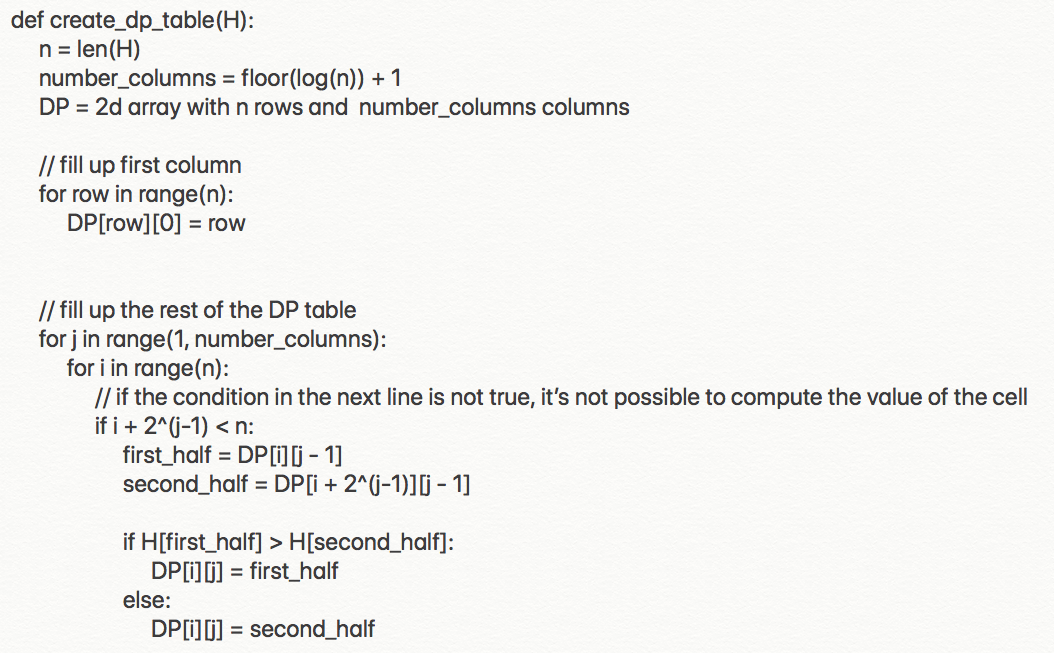
\includegraphics[width=15cm]{2b.png}
\end{figure}
  \\
  \textbf{Runtime:}\\ The first for loop runs in $\mathcal{O}(n)$ and the second and third loops run in a total of $\mathcal{O}(n\log n)$. Everything else runs in constant time, so the total run-time is $\mathcal{O}(n\log n)$.
    \end{enumerate}
    \newpage
    \item % ====== QUESTION 3 =======
    \begin{enumerate}
        \item Create a flow network with the set of vertices $\{s, t, i_1, ..., i_p, j_1, ..., j_m, d_1, ..., d_n\}$. Vertices $i_1, ..., i_p$ represent performances, vertices $j_1, ..., j_m$ represent ringmasters, and vertices $d_1, ..., d_n$ represent days. This flow network should also include the following edges:
        \begin{itemize}
            \item $(s, j_a)$ with capacity $L$ for each $j_a$
            \item $(j_a, i_b)$ with capacity 1 for each ringmaster $j_a$ which can lead performance $i_b$ (i.e., $(j_a, i_b)$ is an edge only if performance $b$ is in the set $P_a$)
            \item $(i_b, d_c)$ with capacity 1 for each performance $i_b$ and day $d_c$
            \item $(d_c, t)$ with capacity $k$ for each day $d_c$
        \end{itemize}
        The algorithm should perform the following on this flow network:
        \begin{itemize}
            \item Compute a maximum flow $f$ via the Ford-Fulkerson algorithm. This returns an integral flow.
            \item Compare $f$ to $n \times k$. If $f < n \times k$, then a schedule which meets the given criteria is impossible. Otherwise, $f = n \times k$, and we found a viable schedule. The flow network can be converted back to a schedule. For any path $j_a, i_b, d_c$ that has a flow of 1, ringmaster $a$ is scheduled to lead performance $b$ on day $c$.
        \end{itemize}
        \item There is a one-to-one correspondence between an integral flow $f$ and an assignment of ringmasters to performances to days in the following way:
        \begin{itemize}
            \item $f(j_a, i_b) = 1$ and $f(i_b, d_c) = 1$ if and only if ringmaster $a$ is scheduled to lead performance $b$ on day $c$
            \item $f(s, j_a)$ is the number of performances ringmaster $a$ is scheduled to lead in total in all $n$ days
            \item $f(d_c, t)$ is the number of performances in day $c$
        \end{itemize}
        \textbf{Correctness.} Since each edge $(s, j_a)$ has a capacity of $L$, no ringmaster can lead more than $L$ performances in total in all of the $n$ days (satisfies constraint 5). Since there is only one edge from each performance $i_b$ to each day $d_c$, a performance can only occur once each day (satisfies constraint 4). This also means that every performance node $i_b$ can have a maximum influx of 1, since $f^{in} = f^{out}$ for every node except $s$ and $t$, meaning each performance has one ringmaster (satisfies constraint 1). Since $(j_a, i_b)$ is an edge only if performance $b$ is in the set $P_a$, a ringleader can only lead a performance they are qualified for (satisfies constraint 2). Since each edge $(d_c, t)$ has a capacity of $k$, if each of these edges has a flow of $k$, $k$ performances will be scheduled on day $c$ (satisfies constraint 3).
        
        \textbf{Running time.} This flow network has $p + m + n + 2$ vertices \\
        and $m + \big(\sum_{j \in \{1, ..., m\}} |P_j|\big) + (p \times n) + n \leq m + (m \times p) + (p \times n) + n$ edges. The sum of the capacities of edges leaving $s$ is $m \times L$. Therefore, the worst-case running time of the naive Ford-Fulkerson algorithm is:
        \begin{align*}
            &\bigO\bigg(m \times L \times \big((p + m + n) + (m \times p) + (p \times n)\big)\bigg) \\
            = &\bigO\bigg(m \times L \times \big((m \times p) + (p \times n)\big)\bigg)
        \end{align*}
    \end{enumerate}
    
    
    
    \newpage
    \item % ====== QUESTION 4 =======
    \begin{enumerate}
        \item Our goal is to find a feasible assignment of staff members to days such that:
        \begin{itemize}
            \item Exactly $a_i$ staff members should be scheduled on day $i$
            \item Each staff member $j$ can only be assigned to a subset of days $A_j \subset \{1, ..., n\}$
            \item Each staff member can be scheduled on at most $L$ days from $A_j$
        \end{itemize}
        \\
        Create a flow network with the set of vertices $\{s, t, d_1, ..., d_n, f_1, ..., f_m\}$\\
        Vertices $d_1, ..., d_n$ represent the $n$ days. Vertices $f_1, ..., f_m$ represent the staff members.\\
        The flow network also has the following edges:
        \begin{itemize}
            \item $(s, d_i)$ with capacity $a_i$ for each $i$
            \item $(d_i, f_j)$ with capacity 1 where $i \in A_j$ for member $f_j$
            \item $(f_j, t)$ with capacity $L$ which is the maximum load a member can have.
        \end{itemize}
        We have reduced the problem to this network flow problem which proceeds as follows:
        \begin{itemize}
            \item Compute a maximum flow $f$ in this network via the Ford-Fulkerson algorithm. Note that it will return an integral flow.
            \item If $f(s, d_i) = a_i$ for each day $d_i$, then a feasible assignment exists. We assign member $f_j$ to day $d_i$ whenever $f(d_i, f_j) = 1$
            \item Otherwise, a feasible assignment does not exist.
        \end{itemize}
        To see that this algorithm is correct, we notice that there is a one-to-one correspondence between an integral flow $f$ and an assignment of staff members to days in the following way:
        \begin{itemize}
            \item $f(d_i, f_j) = 1$ if and only if $f_j$ member is assigned to staff on day $d_i$, and 0 otherwise.
            \item $f(s, d_i)$ is the number of people assigned to each day $d_i$.
            \item $f(f_j, t)$ is the number of days a staff member $f_j$ is assigned to.
        \end{itemize}
        Due to the way the edges are created in the flow network, the second and third constraints in the problem statement are satisfied in the assignment corresponding to any valid flow. Staff members are only assigned to days they can work on and the edge capacity for each member $j$ is $L$, meaning they cannot work more than $L$ days of the $A_j$ possible. Therefore, a feasible assignment exists if and only if the maximum flow $f$ satisfied $f(s, d_i) = a_i$ for each day $d_i$.\\
        \\
        This flow network has $n + m + 2$ vertices and $n + m + \sum^m_{j=1}|A_j| \leq m + n + n \times m$ edges. There are $n$ edges coming out of $s$ and $m$ edges going into $t$. For a given day $d_i$, there can be at most $m$ edges (since that would be all the staff) so, $n \times m$ is an upper bound on the number of edges for the summation.\\
        The sum of capacities of edges leaving $s$ is $\sum^n_{i=1} a_i$. This is $\leq \sum^n_{i=1} m = n \times m$ since we know that at most $m$ people will be assigned to each day.\\
        Hence, the worst-case running time of the naive Ford-Fulkerson algorithm is $\mathcal{O} (n^2 \times m^2)$, which is polynomial in the input length.
        
        \newpage
        \item Our goal is to find a feasible assignment of staff members to days such that:
        \begin{itemize}
            \item Exactly $a_i$ staff members should be scheduled on day $i$
            \item Each staff member can be scheduled on at most $L$ days from $A_j$
            \item Each staff member can be scheduled on at most $L'$ days outside of $A_j$
        \end{itemize}
        \\
        Create a flow network with the set of vertices $\{s, t, d_1, ..., d_n, w_1, ..., w_m, o_1, ..., o_m\}$\\
        Vertices $d_1, ..., d_n$ represent the $n$ days. Vertices $w_1, ..., w_m$ represent the days staff members $j$ are scheduled to work from the days in $A_j$. Vertices $o_1, ..., o_m$ represent the days which staff members $j$ are scheduled to work from the days not in $A_j$.\\
        The flow network also has the following edges:
        \begin{itemize}
            \item $(s, d_i)$ with capacity $a_i$ for each $i$
            \item $(d_i, w_j)$ with capacity 1 where $i \in A_j$ for member $j$
            \item $(d_i, o_j)$ with capacity 1 where $i \not \in A_j$ for member $j$
            \item $(w_j, t)$ with capacity $L$ which is the maximum load a member can have from days in $A_j$.
            \item $(o_j, t)$ with capacity $L'$ which is the maximum load a member can have from days not in $A_j$.
        \end{itemize}
        We have reduced the problem to this network flow problem which proceeds as follows:
        \begin{itemize}
            \item Compute a maximum flow $f$ in this network via the Ford-Fulkerson algorithm. Note that it will return an integral flow.
            \item If $f(s, d_i) = a_i$ for each day $d_i$, then a feasible assignment exists. We assign member $j$ to day $d_i$ whenever $f(d_i, w_j) = 1$ or $f(d_i, o_j) = 1$
            \item Otherwise, a feasible assignment does not exist.
        \end{itemize}
        To see that this algorithm is correct, we notice that there is a one-to-one correspondence between an integral flow $f$ and an assignment of staff members to days in the following way:
        \begin{itemize}
            \item $f(d_i, w_j) = 1$ if and only if $i \in A_j$ and member $j$ is assigned to staff on day $d_i$, and 0 otherwise.
            \item $f(d_i, o_j) = 1$ if and only if $i \not \in A_j$ and member $j$ is assigned to staff on day $d_i$, and 0 otherwise.
            \item $f(s, d_i)$ is the number of people assigned to each day $d_i$.
            \item $f(w_j, t)$ is the number of days a staff member $w_j$ is assigned to from days in $A_j$.
            \item $f(o_j, t)$ is the number of days a staff member $w_j$ is assigned to from days not in $A_j$.
        \end{itemize}
        Due to the way the edges are created in the flow network, the second and third constraints in the problem statement are satisfied in the assignment corresponding to any valid flow. According to the edge capacities, staff members are assigned at most $L$ days to work from $A_j$ and at most $L'$ days to work from outside set $A_j$. Therefore, a feasible assignment exists if and only if the maximum flow $f$ satisfied $f(s, d_i) = a_i$ for each day $d_i$.\\
        \\
        This flow network has $n + 2m + 2$ vertices and $n + 2m + n \times m$ edges. Coming from $s$, there are $n$ edges and from $t$ there are $2m$ edges. In between, for a given $d_i$ day, it is impossible for both $w_j$ and $o_j$ to have an edge with $d_i$ since by definition, $i$ is either in or not in the set $A_j$.\\
        The sum of capacities of edges leaving $s$ is $\sum^n_{i=1} a_i$. This is $\leq \sum^n_{i=1} m = n \times m$ since we know that fewer than m people will be assigned to each day.\\
        Hence, the worst-case running time of the naive Ford-Fulkerson algorithm is $\mathcal{O} (n^2 \times m^2)$, which is polynomial in the input length.
    \end{enumerate}
\end{enumerate}
			
            




\end{document}
